\chapter{Onde in forma fasoriale} 

\begin{figure}[h]
    \centering
    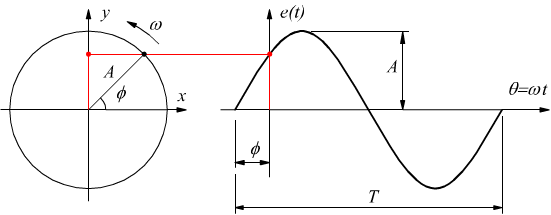
\includegraphics[scale = 0.9]{Fasori rappresentazione.png}
    
\end{figure}

\newpage 

\section{Equazioni dell'onda in forma fasoriale}

\footnote{FWC - pag 135 | 3.10 Uniform plane waves with steady-state sinusoids } 

Prendiamo una componente del campo elettrico, ad esempio $E_x (z,t)$. \\ 
Essenndo una sinusoide, $E_x (z,t)$ possiamo scriverla nella forma: 

{\Large \begin{equation}
    E_x (z,t) = C_1 e^{-\jmath \kappa z} + C_2 e^{\jmath \kappa z}
\end{equation}} 

in cui: 

\begin{itemize}
    \item $C_1$ e $C_2$ sono numeri reali 
    \item $C_1 = E_o ^+  $
    \item $C_2 = E_o ^-  $  
    \item $\kappa = \omega \sqrt{\mu \varepsilon} = \frac{\omega}{v}$
\end{itemize} 

\begin{tcolorbox}
    Dalla matematica, 
    $\omega$ (si legge omega) è la frequenza dell'onda misurata in radianti al secondo [rad/s]. \\ 
    $\omega = 2\pi f$ \\ 
    dove f è la frequenza dell'onda o l'inverso di un periodo misurata in [Hz] (si legge Hertz) o [$\frac{1}{s}$].  \\ \\ 
    
    $\jmath$ è l'unità immaginaria. \\ 
    $\jmath^{2} = -1$ \\ \\ 

    è il numero di Eulero. \\  



    Perchè scrivere le onde in forma fasoriale? \\ \\ 
    Tutto grazie alla formula di Eulero: \\ \\ 
    $e^{\jmath z} = \cos(z) + \jmath \sin(z)$ \\ \\

    Se vuoi approfondire, ci sono due video molto interessanti riguardo al tema: 

    \begin{itemize}
        \item Zech Star - Why do Electrical Engineers use imaginary numbers in circuit analysis? \\ \url{https://youtu.be/FCNHN7B9iDM?si=9ECin22SXTxcp7-6} 
        \item The Science Asylum - What the HECK is a Phasor? Alternating Current Explained. \\ \url{https://youtu.be/7weMCsff0xw?si=Y9t8nKBIX3a1I5Z5}
    \end{itemize}

    

\end{tcolorbox}

$\kappa$ prende il nome di numero d'onda o costante di fase e si misura in $[\frac{1}{m}]$; può essere vista 
anche come la costante del medio per una particolare frequenza (ricordando che $\mu$ e $\varepsilon$ dipendono rispettivamente da $\mu_r$ 
e $\varepsilon_r$ del materiale) \\ 

$E_x (z,t)$ è una funzione che dipende sia da z (nell'asse cartesiano) che da t (cioè il tempo).  \\ \\

Essa è la somma di un'onda progressiva, cioè un'onda lungo z, che viene indicata dalla notazione $E_o ^+ e^{-\jmath \kappa z}$ 
e di un'onda regressiva, cioè un'onda lungo -z, che viene indicata dalla notazione $E_o ^- e^{\jmath \kappa z}$ \\ 

$E_o ^+ e^{-\jmath \kappa z}$ diventa negativa lungo l'asse z, con velocità v, mentre $E_o ^- e^{\jmath \kappa z}$ dievnta positiva 
lungo l'asse -z con velocità -v. \\ \\ 

Moltiplicando l'equazione per $e^{\jmath \omega t}$, è possibile convertirla in coordinate cartesiane e sapere come l'onda varia nel tempo:

{
    \Large
    \begin{equation}
        \begin{split}
            E_x (z,t) 
            &= \mathfrak{Re}[E_x e^{\jmath \omega t}]\\ 
            &= \mathfrak{Re}[C_1 e^{- \jmath \kappa z} e^{\jmath \omega t} +  C_2 e^{ \jmath \kappa z} e^{\jmath \omega t}]            
        \end{split}
    \end{equation}
}


Prendendo $C_1$ e $C_2$ come reali, avremo che: 

{
    \Large
    \begin{equation}
    E_x (z,t) = C_1 \cos(\omega t - \kappa z) + C_2 \cos(\omega t + \kappa z)    
    \end{equation}
}

Ricordando che: 
{
    \Large
    \begin{equation}
        \kappa = \frac{\omega}{v}   
    \end{equation}
}

possiamo scriverla anche come: 
{
    \Large 
    \begin{equation}
    E_x (z,t) = C_1 \cos\omega( t - \frac{z}{v}) + C_2 \cos\omega( t + \frac{z}{v})
    \end{equation}
}

Nello scorso capitolo, le equazioni di Maxwell in forma fasoriale, abbiamo scoperto che:  
{
    \Large
    \begin{equation}
     \nabla \times \vec{E} = -\jmath \omega \mu \vec{H}   
    \end{equation}
}


Nell'asse y sappiamo la relazione tra $E_x$ e $H_y$:  

{
    \Large
    \begin{equation}
    \frac{\partial E_x}{\partial z} = -\jmath \omega \mu H_y     
    \end{equation}
}

Dividendo l'equazione per $-\jmath \omega \mu$, possiamo trovare $H_y$: 
{
    \Large
    \begin{equation}
   H_y = - \frac{1}{\jmath \omega \mu} \frac{\partial E_x}{\partial z }     
    \end{equation}
}

Ricordando che: 

{
    \Large
    \begin{equation}
   E_x (z,t) = C_1 e^{-\jmath \kappa z} + C_2 e^{\jmath \kappa z}     
    \end{equation}
}


$H_y$ possiamo scriverla come: 

{
    \Large
    \begin{equation}
   H_y = \frac{\kappa}{\omega \mu} [E_o ^+ e^{-\jmath \kappa z} - E_o ^- e^{\jmath \kappa z}]     
    \end{equation}
}

Sviluppando l'equazione, avremo che: 
{
    \Large 
    \begin{equation}
   H_y = \sqrt{\frac{\varepsilon}{\mu}} [E_o ^+ e^{-\jmath \kappa z} - E_o ^- e^{\jmath \kappa z}]      
    \end{equation}
}


In forma instantanea, $H_y$ la possiamo scrivere come: \\ 

{
    \Large
    \begin{equation} 
        \begin{split}
            H_y (z, t) 
            &= \mathfrak{Re}[H_y(z) e^{\jmath \omega t}] 
            \\
            &= \frac{1}{\sqrt{\frac{\mu}{\varepsilon}}}[E_o^+ \cos(\omega t - \kappa z) - E_o^- \cos(\omega t + \kappa z)]  
        \end{split}
    \end{equation}
}
dove: 

{
    \Large
    \begin{equation}
        \sqrt{\frac{\mu}{\varepsilon}} = \eta     
    \end{equation}
}

$\eta$ (si legge eta) prende il nome di impedenza d'onda. \\ \\ 

Ritornando all'esempio nel piano in z=0, \\ \\ 

{\Large \begin{equation}
    \begin{cases}
        E_x (z) = -2 \jmath E_0^+ \sin(\kappa z) \\ \\ 
        H_y (z) = 2 \frac{E_0^+}{\eta} \cos(\kappa z)
    \end{cases}
\end{equation}} \\ 

Da queste due equazioni finali, notiamo che $E_x (z)$ e $H_y (z)$ sono in quadratura 
di fase, cioè sono sfasati di 90° \\ \\ 

\begin{figure}[h]
    \centering 
    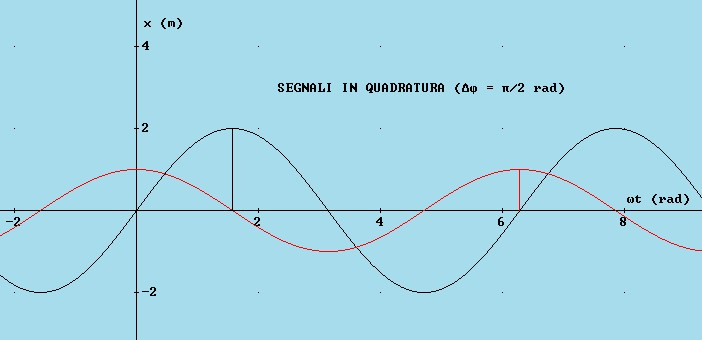
\includegraphics[scale = 0.8]{InQuadratura.jpg} 
    
\end{figure} 

\footnote{Wikipedia - Fase (Fisica)} \\ 

Per riassumere, usando le leggi di Maxwell per le onde piane, possiamo scriverle anche come: \\ 

{\Large \begin{equation}
    \begin{cases}
        \nabla ^{2} \vec{E} = -\kappa ^{2} \vec{E} \\ 
        \nabla ^{2} \vec{H} = -\kappa ^{2} \vec{H}
    \end{cases}
\end{equation}} 

dove: 
{
    \Large
    \begin{equation}
    \kappa ^{2} = \omega ^{2} \mu \varepsilon    
    \end{equation}
}

\newpage 








